\chapter{Traffic simulator}

We created a traffic simulator for the testing of platooning concept and cooperation of vehicles in platoons. For verification and testing of our assumptions and theories we had to set up a simulation environment which tries to compare real traffic transport statistics with general driver’s behaviour. We did not find an adequate simulator which would satisfy our needs (response time, flexibility, user modifiability, customisability), so we had to create a new one. In this part we will describe our used simulation environment and its features which affected our tests. 

For creation of multi-agent simulation scenarios we use and customize the simulation toolkit Alite that is also used for some projects inside AgentDrive platform developed by Agent Technology Centre in CTU.





\section{Alite and AgentDrive platform simulations}

The Alite is an agent-based simulation toolkit for multi-agent systems which corresponds to our need for big traffic simulation of independent vehicles. All description of project Alite can be found on its websites\footnote{\url{http://jones.felk.cvut.cz/redmine/projects/alite/wiki/Alite_Overview}}\cite{schaefer2011}.

The original composition of AgentDrive (which is based on Alite simulator) simulation mostly consists of two parts which have event based communication. The main part of the program – Highway module - contains all data of simulation and agents and it sends events and data into the second part - Simulator Lite - where graphical visualization is realized and physical simulation is also done. The Simulator Lite sends back the information about the actually changed positions of all objects depending on the physical aspects such as acceleration or maximum steering angle and so on. 

The agents then react on the changed positions and Highway module again sends new agent’s actions into simulator, such as the way-point where the adequate object (agent vehicle) should go. In the base implementation there was only an agent called RouteAgent which was able to follow its way and slow down in curves but it was not able to react to other agents.

\section{Our main improvements}

In source code of used simulator we had to do several changes with the graphical visualisation routines of highway simulation module to be able to realise and verify our assumptions. In this chapter there are descriptions of the main modifications to which we refer in next chapters and which set basic features of our highway simulator.

Since we use a big amount of vehicles (thousands of units), we decided not to use graphical visualisation of Simulator Lite , but to use only simulation functions of Simulator Lite and to use default visualisation in  Highway module. In Simulator Lite some time delays appeared in comparison with real time, because of compression and decompression of big quantity of commands. We could omit the physical model, because we assume straight or slightly curved highways and acceleration and deceleration of cars is included in vehicle-agent behaviour. 

We also add a possibility to define and simulate passenger vehicles (cars) and trucks, two main types of traffic participants. These two types are different in length and have several different characteristics. The speed of the cars is various according to the car speed Gaussian distribution, but trucks use defined limit speed and both the vehicle types have also a little different behaviour (see more details in next chapters).

\subsection{Java class: PlatooningAgent}

PlatooningAgent is derived from default RouteAgent which only follows generated predefined way-points. The instance holds basic information about the agent as a vehicle, it has different braking acceleration coefficients for dry, wet and snowy weather as well as information about index of lane in which the agent is.  We also added next abilities and features: 

\begin{itemize}
\item Counting Breaking coefficient - This feature returns breaking coefficient according to defined safety conditions.
\item Speeding up, acceleration – Agent can increase its actual speed up to its defined maximum value. The speed growth is directly proportional to the acceleration time. At this moment we use the same coefficient for acceleration and deceleration depends on safety conditions.
\item Slowing down, deceleration – It is very similar to Speeding up feature, but in opposite direction, value is going down to the limit 0 m/s.
\item Changing lanes – this function actively controls changing of lanes.  
\end{itemize}

\subsection{Java class: VehicleGenerationModule}

It could be expected that the Module generates vehicles only in the right highway lane and into the left lane the vehicle moves by overtaking and changing of lane, as it is usual by standard driver’s behaviour after the car is starting on highway by using a highway entrance ramp lane. But it is not true for our traffic simulator scenarios, because we simulate an existing traffic, so the Module generates agents in each  lane (according to vehicle type), even in the left lane.

This module works as the statistic centre for generation of new vehicles, it does not create new agents. According to statistic data it provides information whether a new vehicle should be generated there or not. It reads next entry parameters from platooning.groovy configuration file, in section platooning.VehiclesGenerationModule:

\begin{itemize}
\item	\textit{Generation limit} [Boolean] – Parameter decides either to use the Total number of vehicle per hour limit parameter or to generate as many vehicles as it is possible, it means to  generate another vehicle every time if  there is enough space to position it on highway.
\item	\textit{Total number of vehicles per hour} [Integer] - It is a maximum number of vehicles which should be generated in one hour in case there is enough space to generate them. Other vehicles can be added only if the ratio of total number of generated vehicles and time from the start of simulation is lower than this parameter.  
\item \textit{Passenger vehicle ratio} [Float] – Necessary only if value Simulator Lite \textit{Generate trucks} is true. It is number between 0 and 1 which corresponds to the percentage of passenger vehicles in  the number of all generated vehicles.
\item \textit{Average speed and Speed dispersion} [Float] – by these two parameters the speed Gaussian distribution of cars on highway is influenced.
\item \textit{Minimum speed} [Float] – Minimum vehicle speed limit is set.
\item \textit{Ratio of platoon vehicles} [Float] – Number from interval 0 to 1 which corresponds to how many percent of passenger vehicles should be placed in platoons.
\item \textit{Maximum length of platoon} [Integer] – Corresponds to maximum number of following vehicles in platoon. VehiclesGenerationModule generates platoons with number of following vehicles by Uniform distribution from 2 to this parameter.
\item \textit{Generate trucks} [Boolean]– This parameter decides whether to add or not a trucks to the simulation.
\item \textit{Truck speed} [Boolean] – It is a speed that is common for all generated trucks.
\end{itemize}


It is possible to set up these parameters variously , but for realistic simulation it is recommended to see Chapter 2.




\subsection{Java class: PlatooningCenterModule}

This obejct is responsible for traffic safety, it also contains all main platooning logic and agents’ decisions. We decided to centralize all logic and variant decisions into this location instead of to the agent class, because then it is easier to do changes and to debug the progress. After the platooning concept is finished, the concept can be easily moved to PlatooningAgent class.

This class is responsible for adding new vehicles into simulation, for changing of speed and lane of agents and for printing statistic information into external file for subsequent evaluation. 

\subsubsection{Passenger vehicles and trucks}

PlatooningCentreModule adds passenger vehicles or trucks according to information from VehicleGenerationModule. All vehicles (cars and trucks) can be formed now into platoons (in the past it was possible only with cars). They have their own \textit{Preferred speed}. It means that each vehicle has its own speed that it prefers to drive and its actual speed equals to this \textit{Preferred speed} or it is lower. 

Both types of vehicles (cars and trucks) differ in some of their properties.

Passenger vehicle:

\begin{itemize}
\item \textit{Preferred speed} of agent is generated in VehicleGenerationModule according to the Gaussian distribution influenced by parameters \textit{Average speed} and \textit{Speed dispersion}, agents have different \textit{Preferred speed}.
\item Agent can be generated and starts in every lane.
\item Agent can change lanes during simulation.
\end{itemize}

Truck:

\begin{itemize}
\item \textit{Preferred speed} of agent equals to parameter \textit{Truck speed}, all truck agents have the same \textit{Preferred speed}
\item Agent can be generated and starts only in right lane.
\item Agent cannot change lane during simulation
\end{itemize}

\subsubsection{Distance conditions}

In order to make the traffic in simulator safety, we set up some rules which are based on following definitions:

\begin{itemize}
\item \textit{Reaction distance} – $s_r$ – Distance that a vehicle travels during simulator response time (it waits for simulator back event). This distance would be important especially for simulator with high response time.

For $t_{sim}$ is run time period of simulator, that is defined as 0.1 second, and $v$ is speed of vehicle

\begin{equation}
s_{r}=t_{sim}\cdot v\label{eq:sr}
\end{equation}

\item \textit{Safe time distance} - $s_{std}$ -  it corresponds to distance which vehicle travelled over Safe time by its speed. Safe time\footnote{\url{https://www.gov.uk/general-rules-all-drivers-riders-103-to-158/control-of-the-vehicle-117-to-126}} – $t_{s}$ is a recommended time which should be between two vehicles going at the same speed, so the back driver is able to react a dangerous distance to the front car. Minimal recommended value is 2 seconds (you can also find it as “2 second rule”). Safe time is set in our simulator to 2 seconds too. We select this minimal value, because we would like to maximize  the highway traffic. For vehicle speed $v$:

\begin{equation}
s_{std}=t_{s}\cdot v=2\cdot v\label{eq:std}
\end{equation}

\item \textit{Slow down distance} – $s_{sdd}$ – Distance which is needed to slow down the back vehicle to the speed of the vehicle going ahead. When the front vehicle is faster than the back one, this distance is equal to zero.

For back vehicle speed $v_b$, front vehicle’s speed $v_f$ and deceleration $a_b$ of back vehicle:

\begin{equation}
v_{b}>v_{f\:}:\:s_{sdd}=\frac{v_{b}\cdot(v_{b}-v_{f})}{a_{b}}-\frac{0.5\cdot(v_{b}-v_{f})^{2}}{a_{b}}\label{eq:ssdd}
\end{equation}

\item \textit{Different speed correction} - $c_{ds}$ – is a value that corresponds to quadrat of difference of back vehicle speed and front vehicle speed. This value can equal maximally to 40\% (we used this value for the thesis, but it can be set in setting file of simulator) for this thesis of \textit{Safe time distance} of the back vehicle. The correction serves as an indicator of how much can a vehicles disrupt a \textit{Front safe distance} (described lower) of a overtaken vehicle.

For the back vehicle speed - $v_b$, the front vehicle speed $v_f$, back vehicle \textit{Safe time distance} - $s_{stdb}$:

\begin{equation}
c_{ds}=min(0.4\cdot s_{stdb},\frac{(v_{f}-v_{b})^{2}}{min(v_{f},v_{b})}\cdot s_{stdb})\label{eq:cds}
\end{equation}

\end{itemize}

\subsubsection{Safe behaviour of vehicles in simulator}

The Platooning module is responsible for safe traffic. To achieve this goal we had to set up some rules which must be respected by all vehicles in the traffic.

\paragraph{\textit{Front safe distance}}

Each vehicle must maintain a sufficient distance from the vehicle that goes ahead, to have time to react. \textit{Front safe distance} of \textit{\mbox{Vehicle 1}} in a lane is minimum distance which should be free in front of this vehicle to avoid unnecessary actions.

In our simulator, this \textit{Front safe distance} consists of sum of \textit{Safe time distance} of \textit{\mbox{Vehicle 1}}, \textit{Slow down distance} of \textit{\mbox{Vehicle 1}} - \textit{\mbox{Vehicle 2}} (which is the closest front vehicle in its lane) and \textit{Reaction distance} as you can see in Figure \ref{fig:4_2_3_3-1}

\begin{figure}[ph]
\centering
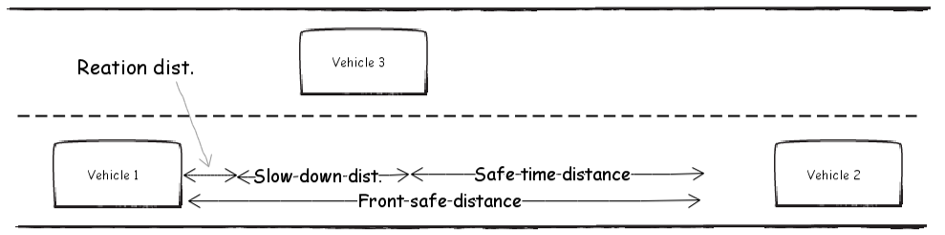
\includegraphics[width=0.90\textwidth,height=0.90\textheight,keepaspectratio]{figures/Chapter_4/4_front_safe_distance.png}
\centering
\protect\caption{\label{fig:4_2_3_3-1}\textit{Front safe distance} of \textit{\mbox{Vehicle 1}} to the closest front \textit{\mbox{Vehicle 2}}}
\end{figure}

For example with \textit{\mbox{Vehicle 1}} \mbox{speed  = 30 m/s},  \textit{\mbox{Vehicle 2}} \mbox{speed = 28 m/s}, braking acceleration = \mbox{4 m/$s^2$} and simulator iteration \mbox{time = 0.1} s then \textit{Front safe distance} of \textit{\mbox{Vehicle 1}}  is \mbox{77.5 m}. If the distance between \textit{\mbox{Vehicle 1}} and \textit{\mbox{Vehicle 2}} is smaller \textit{\mbox{Vehicle 1}} has to react on this situation.

If the front \textit{\mbox{Vehicle 2}} is faster at least 1 m/s (ex. 31m/s) than back \textit{\mbox{Vehicle 1}}, \textit{Slow down distance} will be equal 0, as we mentioned before. Because the \textit{\mbox{Vehicle 2}}  is faster than \textit{\mbox{Vehicle 1}} the \textit{Safe time distance} is decreased to 80\% to avoid pointless actions (slowing down \textit{\mbox{Vehicle 1}}, the real distance between \textit{\mbox{Vehicle 1}} and \textit{\mbox{Vehicle 2}}   is less than \textit{Front safe distance}; more about the behaviour rule in part Vehicle behaviour in this section).  \textit{Safe time distance} could be reduced, because then \textit{\mbox{Vehicle 2}} is faster and therefore real \textit{Front safe distance} will be increasing in time and probability of crash is minimal.

According to observation of real traffic we added an exception for case that the front \textit{\mbox{Vehicle 2}} is truck, then the \textit{Safe time distance} is reduced to 40\% of normal distance, because truck braking path is longer than that of the car.

\paragraph{\textit{Overtaking distance}}

is distance that the overtaking vehicle (\textit{\mbox{Vehicle 1}}, Figure \ref{fig:4_2_3_3-2}) must be in front of the overtaken vehicle (\textit{\mbox{Vehicle 2}}) to be able to safely change into the lane (\textit{\mbox{Vehicle 2}} lane). This distance defines, how far the vehicle should be to overtake the back vehicle in dependency of their speed difference.

\begin{figure}[ph]
\centering
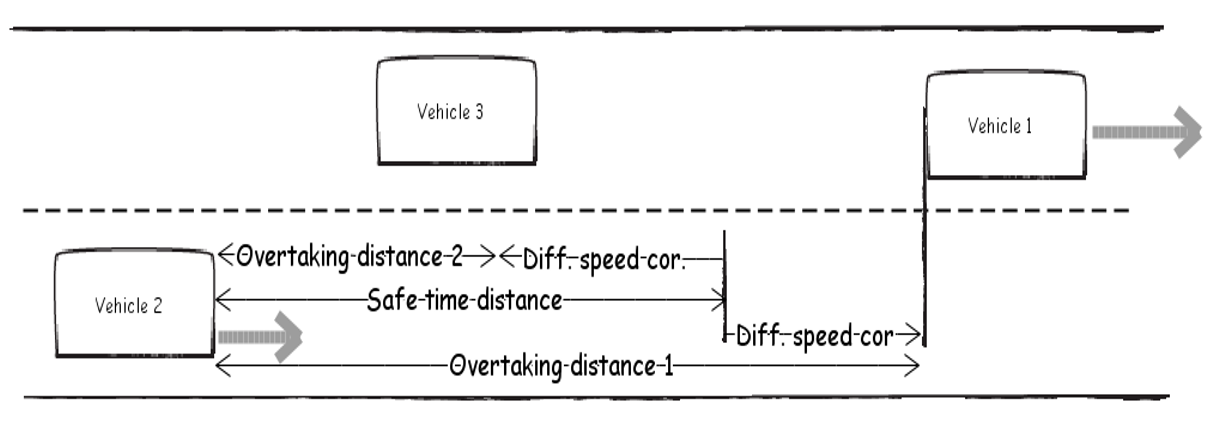
\includegraphics[width=0.90\textwidth,height=0.90\textheight,keepaspectratio]{figures/Chapter_4/4_overtaking_distance.png}
\centering
\protect\caption{\label{fig:4_2_3_3-2}\textit{Overtaking distance} of \textit{\mbox{Vehicle 1}} to closest back vehicle in lower lane \textit{\mbox{Vehicle 2}}}
\end{figure}

As you can see in Figure \ref{fig:4_2_3_3-2}, \textit{Overtaking distance} of \textit{\mbox{Vehicle 1}} at destined lane (in that figure it is in the right lane) consists of \textit{Safe time distance} of the closest back \textit{\mbox{Vehicle 2}} in the lane and Difference speed correction. \textit{Different speed correction} is added to the \textit{Safe time distance} if \textit{\mbox{Vehicle 1}} is slower than \textit{\mbox{Vehicle 2}}. Otherwise the \textit{Safe time distance} is decreased by the \textit{Different speed correction}. 

So in Figure \ref{fig:4_2_3_3-2}, \textit{Overtaking distance} of \textit{\mbox{Vehicle 1}} from \textit{\mbox{Vehicle 2}} is \textit{Overtaking distance} 1, if \textit{\mbox{Vehicle 1}} is faster than the closest back \textit{\mbox{Vehicle 2}}. Whether \textit{\mbox{Vehicle 1}} would be slower than \textit{\mbox{Vehicle 2}}, the \textit{Overtaking distance} of \textit{\mbox{Vehicle 1}} in right lane from \textit{\mbox{Vehicle 2}} would be \textit{Overtaking distance} 2. This situation appears in case of unusual \textit{\mbox{Vehicle 1}} driver’s behaviour in overtaking movement, when he does not respect safety rules.

\paragraph{Changing of lane}

- Every vehicle can change lane, but it cannot endanger itself and the others by this action, so there has to be free safety space. The vehicle changing lane can move in space between two other vehicles in the target lane only if next two conditions are met.

\begin{enumerate}
\item The space in front of the changing vehicle in target lane must be bigger than its \textit{Front safe distance}.
\item There has to be free back space to the vehicle in the lane which is bigger as \textit{Overtaking distance} of the changing vehicle.
\end{enumerate}

You can see the conditions in the following Figure \ref{fig:4_2_3_3-3}. In this figure you can see main \textit{\mbox{Vehicle 1}} in \textit{lane 1} with the conditions for changing of lane. You can see that \textit{\mbox{Vehicle 1}} cannot turn to \textit{lane 2}, although its \textit{Front safe distance} is smaller than the distance to the closest front \textit{\mbox{Vehicle 5}} in the \textit{lane 2}  but  \textit{\mbox{Vehicle 1}} \textit{Overtaking distance} is smaller than the distance to \textit{\mbox{Vehicle 4}}. On the other side \textit{\mbox{Vehicle 1}} can turn to \textit{lane 0} because its \textit{Overtaking distance} and \textit{Front safe distance} are smaller than both distances to the closest back \textit{\mbox{Vehicle 2}} and front \textit{\mbox{Vehicle 3}} in \textit{lane 0}.

\begin{figure}[ph]
\centering
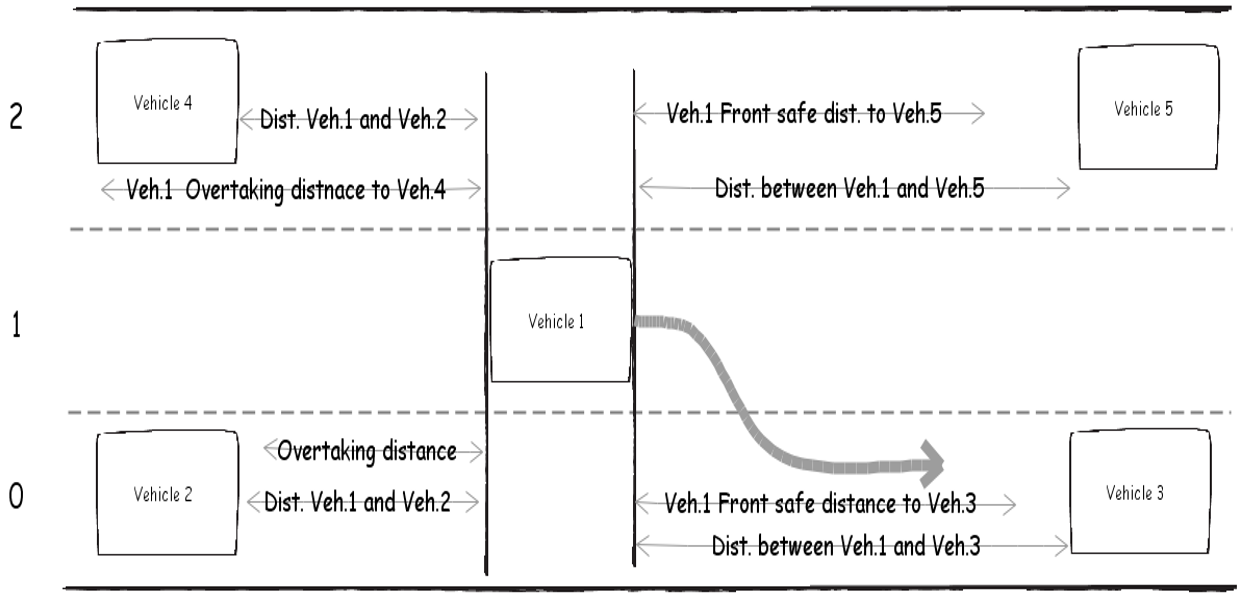
\includegraphics[width=0.90\textwidth,height=0.90\textheight,keepaspectratio]{figures/Chapter_4/4_changing_lanes.png}
\centering
\protect\caption{\label{fig:4_2_3_3-3}Possibilities of \textit{\mbox{Vehicle 1}} to change lane and vehicles which can influence the it}
\end{figure}

During the changing of lane, \textit{Preferred speed} of changing vehicle is modified too. If a vehicle turns to left lane, to the faster one, its speed is increased by 1 m/s. For turning to right lane, to slower one, its speed is decreased by the same value.

\paragraph{Behaviour of vehicles}

- According to the situation on the highway, regular vehicle which is not part of a platoon has 4 options to do, as you can see in decision tree in Figure \ref{fig:4_2_3_3-4} :

\begin{itemize}
\item Speed up, but maximally to its \textit{Preferred speed} and stay in the lane, 
\item Slow down and stay in the lane,
\item Turn to the left lane and speed up, 
\item Turn to the right lane. 
\item Continue without any actions. 
\end{itemize}

\begin{figure}[ph]
\centering
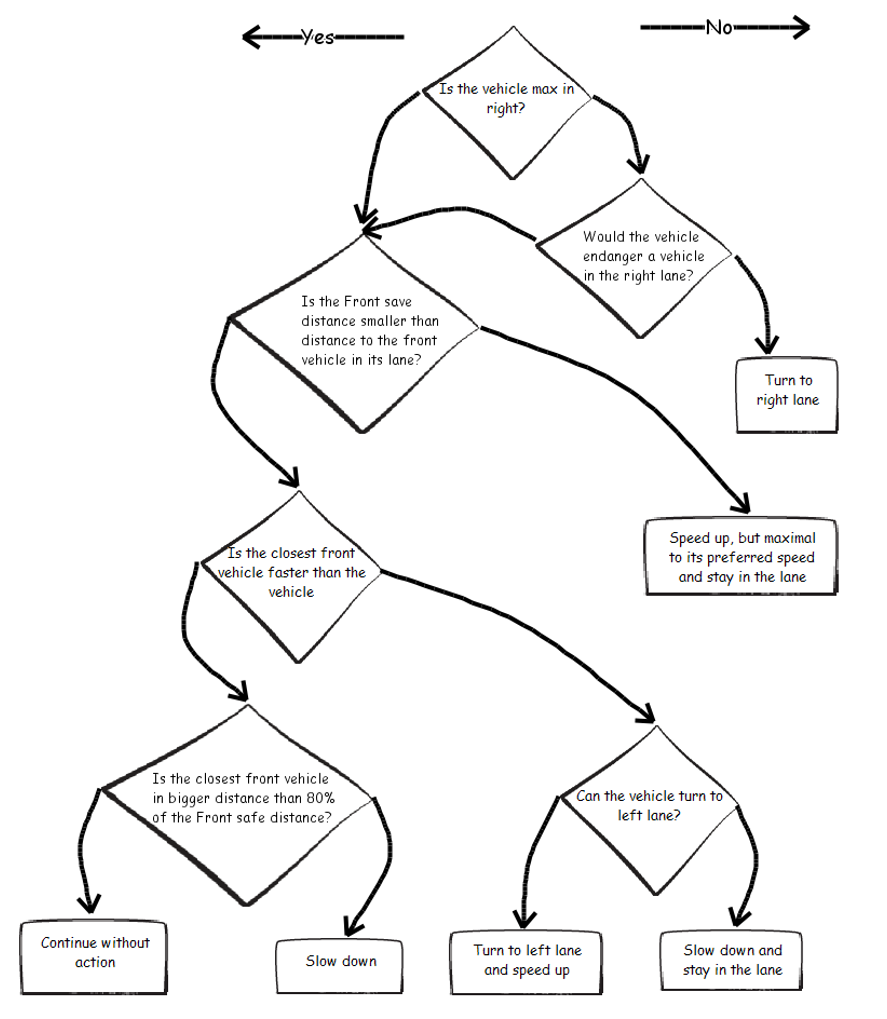
\includegraphics[width=0.95\textwidth,height=0.95\textheight,keepaspectratio]{figures/Chapter_4/4_diagram.png}
\centering
\protect\caption{\label{fig:4_2_3_3-4}Decision diagram of behaviour of passenger vehicle agent in simulator}
\end{figure}

The first rule which every vehicle should observe is to drive on the right side according to Czech law. So if the situation allows it, every vehicle turns to right lane and travels there. This movement is called Changing to slower lane and you can see it in Figure \ref{fig:4_2_3_3-5}. In this example you can see that \textit{\mbox{Vehicle 1}} can according to rule Changing of lane turn to right lane.

\begin{figure}[ph]
\centering
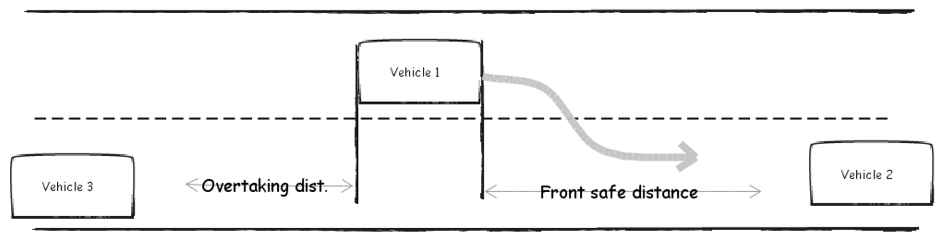
\includegraphics[width=0.90\textwidth,height=0.90\textheight,keepaspectratio]{figures/Chapter_4/4_changing_slower_lane.png}
\centering
\protect\caption{\label{fig:4_2_3_3-5}Situation when \textit{\mbox{Vehicle 1}} can turn to slower lane between \textit{\mbox{Vehicle 2}} and \textit{\mbox{Vehicle 3}}}
\end{figure}

The second rule is to keep preferred speed by overtaking.  As we mentioned before, every vehicle has its \textit{Preferred speed} and tries to stay at this speed level most of the time, so if it can increase its speed to this level, it does it so and this is the second main rule for behaviour of every vehicle. In order to achieve this speed level the vehicle changes its lane to the faster one to avoid its deceleration by some vehicle which goes in front of it in the same lane. This action is called overtaking see in Figure \ref{fig:4_2_3_3-6}. In this example let’s assume that \textit{Vehicles 1}  speed is higher than \textit{\mbox{Vehicle 2}} speed. The distance between these two vehicles in time becomes smaller than the \textit{Front safe distance} of \textit{\mbox{Vehicle 1}} to \textit{\mbox{Vehicle 2}},  then \textit{\mbox{Vehicle 1}} should decide. It prefers overtaking to decelerating and therefore \textit{\mbox{Vehicle 1}} does the overtaking movement to the left lane, respecting Changing of lane condition.

\begin{figure}[ph]
\centering
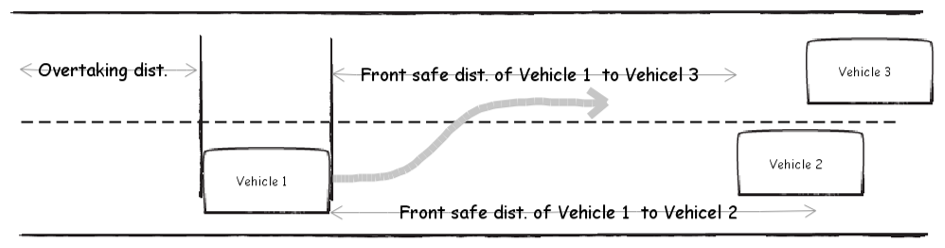
\includegraphics[width=0.90\textwidth,height=0.90\textheight,keepaspectratio]{figures/Chapter_4/4_can_overtake.png}
\centering
\protect\caption{\label{fig:4_2_3_3-6}Situation when \textit{\mbox{Vehicle 1}} can overtake Vehicle\-2 and turn to faster lane behind \textit{\mbox{Vehicle 3}}}
\end{figure}

The next rule is to drive safely by keeping \textit{Front safe distance}. If in front of the vehicle, let us call it \textit{\mbox{Vehicle 1}}, there is another vehicle, \textit{\mbox{Vehicle 2}}, whose speed is smaller than that of \textit{\mbox{Vehicle 1}} and that \textit{\mbox{Vehicle 1}} cannot overtake, \textit{\mbox{Vehicle 1}} has to decrease its speed according to the safe distance in the lane. Like example in Figure \ref{fig:4_2_3_3-7}, which is very similar to previous example, instead of that, the distance between \textit{\mbox{Vehicle 1}} and \textit{\mbox{Vehicle 3}} is smaller than the \textit{Front safe distance} of \textit{\mbox{Vehicle 1}} to \textit{\mbox{Vehicle 3}}. So according to safety rule of Changing of lane, \textit{\mbox{Vehicle 1}} cannot overtake and has to slow down.

\begin{figure}[ph]
\centering
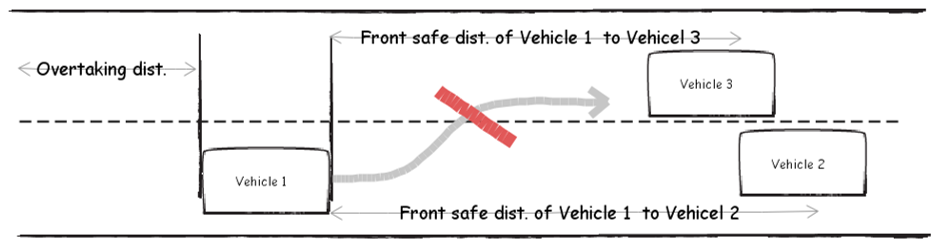
\includegraphics[width=0.90\textwidth,height=0.90\textheight,keepaspectratio]{figures/Chapter_4/4_cannot_overtake.png}
\centering
\protect\caption{\label{fig:4_2_3_3-7}Situation when \textit{\mbox{Vehicle 1}} cannot overtake \textit{\mbox{Vehicle 2}} and turn to faster lane behind \textit{\mbox{Vehicle 3}}}
\end{figure}

\subsection{Platooning}

The PlatooningCentreModule, as the name refers, is responsible for platooning concept. Similarly as it is in VehicleGenerationModule, platoons are also generated in every lane (according to vehicle type) and only at beginning of simulation. They are not created during simulation from single vehicles if the vehicles sequence is changed because of overtaking and changing lanes. And it is not allowed to add vehicle into platoon during simulation. But the platoons could decomposite because of other vehicle drivers' behaviour.

It is not allowed to create a platoon from vehicles, which are already in another one. The number of following vehicles in platoon is generated from VehicleGenerationModule data according to a uniform distribution in interval from 0 to set parameter.

In this thesis we do not deal with internal control system between vehicles in platoon, such as keeping constant distance and speed between vehicles, turning of vehicles, behaviour features, etc. For this work we assume full-functioning platooning model and we test higher highway traffic principles and platoons are part of this traffic as one “entity”. 

Platoons are implemented by one main lead vehicle and many following vehicles. The lead vehicle is responsible for platoon behaviour and influences behaviour of all following vehicles in platoon. It decides about platoon behaviour and sends platoon orders to the rest of the vehicles in platoon. They fulfil this platoon orders of their lead vehicles. Every order contains what the vehicle should do and the location where the order should be filled. The following vehicles independently keep nearly constant distance from the lead vehicle, they speed up or down a little if the distance is bigger or smaller than the required one.

There are implemented three types of changing of lane by platoon:

\begin{itemize}
\item Snake

If the lead vehicle finds out, that it will overtake, it sends platoon order to change lane in the fix location, it means in the same location as the lead vehicle did, in location that lead vehicle decided to change lane, to overtake front vehicle. It is displayed in Figure \ref{fig:4_2_3_3-8}. You can see that this action depends only on \textit{Front safe distance} in the lane and \textit{Overtaking distance} of lead vehicle \textit{\mbox{Vehicle 1}}.

\begin{figure}[ph]
\centering
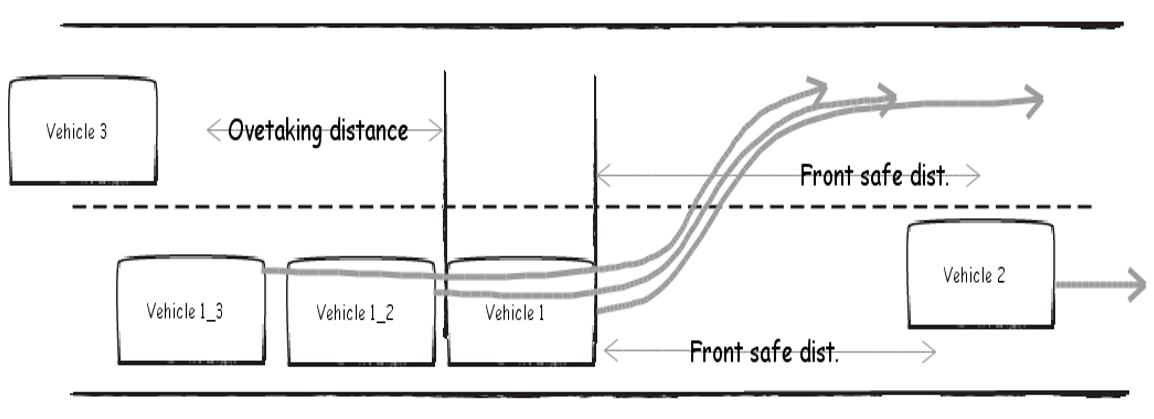
\includegraphics[width=0.90\textwidth,height=0.90\textheight,keepaspectratio]{figures/Chapter_4/4_overtaking_snake.png}
\centering
\protect\caption{\label{fig:4_2_3_3-8}Platoon overtaking type: Snake}
\end{figure}

\item All at once

It is more cooperative approach, all (leading and following) vehicles change a lane at the same time. A platoon starts overtaking action, if there is no vehicle in space defined by position of last platoon vehicle minus its \textit{Overtaking distance} and position of lead vehicle plus its \textit{Front safe distance}. See Figure \ref{fig:4_2_3_3-9}.

\begin{figure}[ph]
\centering
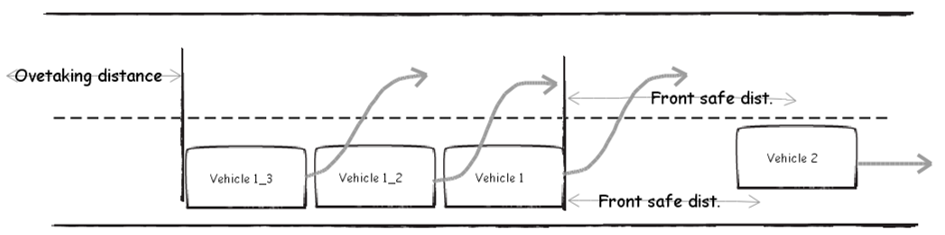
\includegraphics[width=0.90\textwidth,height=0.90\textheight,keepaspectratio]{figures/Chapter_4/4_overtaking_allatonce.png}
\centering
\protect\caption{\label{fig:4_2_3_3-9}Platoon overtaking type: All at once}
\end{figure}

\item Last first - All at once with preparation

If the platoon cannot change lane by All at once , the Change of lane movement is realized in two steps, as you can see in Figure \ref{fig:4_2_3_3-10}. The first step is change of lane only by the last platoon \textit{\mbox{Vehicle 1 3}} to get free space in the lane for rest of the platoon vehicles, potentially to slow down \textit{\mbox{Vehicle 4}} if it is fast one but far. In the figure you can see, that in this step \textit{\mbox{\mbox{Vehicle 1}}} cannot do overtaking movement because of \textit{\mbox{Vehicle 3}}. 

But \textit{\mbox{Vehicle 3}} drives faster than the platoon of \textit{\textit{\mbox{\mbox{Vehicle 1}}}} and step two is realised in some seconds later as you can see in Figure \ref{fig:4_2_3_3-11}, and where also the rest of platoon vehicles can do overtaking movement.

\begin{figure}[ph]
\centering
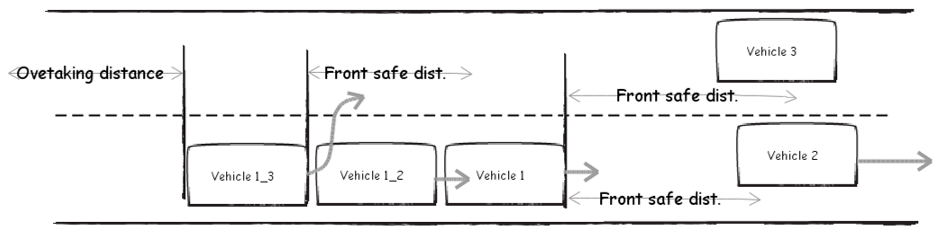
\includegraphics[width=0.90\textwidth,height=0.90\textheight,keepaspectratio]{figures/Chapter_4/4_overtaking_lastFirst1.png}
\centering
\protect\caption{\label{fig:4_2_3_3-10}Platoon overtaking type: Last First - step 1}
\end{figure}


\begin{figure}[ph]
\centering
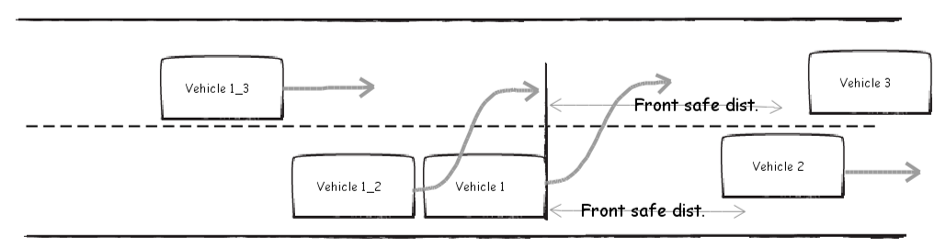
\includegraphics[width=0.90\textwidth,height=0.90\textheight,keepaspectratio]{figures/Chapter_4/4_overtaking_lastFirst2.png}
\centering
\protect\caption{\label{fig:4_2_3_3-11}Platoon overtaking type: Last first - step 2}
\end{figure}


\end{itemize}

\subsubsection*{Collisions during overtaking}

Snake type of overtaking depends only on the Lead vehicle of the platoon and does not depend on location of rest following vehicles in the platoon. In real situation , if  some following vehicle in the  platoon gets to close to another vehicle, this following  vehicle has to leave the platoon and becomes Lead vehicle of a new platoon- see Figure \ref{fig:4_2_3_3-12}.

\begin{figure}[ph]
\centering
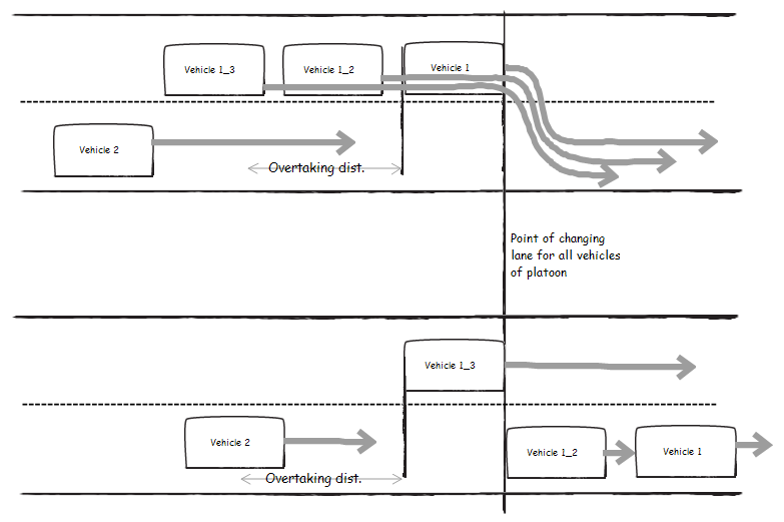
\includegraphics[width=0.90\textwidth,height=0.90\textheight,keepaspectratio]{figures/Chapter_4/4_platoon_decomposition.png}
\centering
\protect\caption{\label{fig:4_2_3_3-12}Conditions and process of decomposition of a platoon}
\end{figure}







\section[Main features of traffic situation measured during the simulation]{Main features of traffic situation measured \newline during the \mbox{simulation}\sectionmark{Main features of traffic...}}
\sectionmark{Main features of traffic...}

There are many features which can be studied. We decided to focused on some, which seemed important to us. There is a list of features, which are predefined in the simulator to be measured.

\begin{itemize}
\item Density of traffic – is the number of vehicles that pass a defined highway in a point per time period without breaking any safety rules that are set in our simulator. This point is at the beginning of simulated part of highway, because the agents (vehicles, platoons) are added only in this point. It is counted as ration of number of all generated vehicles and total time of simulation. To achieve maximum capacity it is necessary to set \textit{Generation limit} to false (parameter is mentioned in Section 4.2.2).
\item Average speed of all vehicles 
\item Average speed of all passenger vehicles
\item Total speed dispersion
\item Average speed of vehicles in each lane
\item Speed dispersion in each lane
\item Actual number of placed vehicles in highway – it is number of vehicles that are “going” in highway at that moment, at the time
\item Actual number of placed vehicles in each lane
\item Frequency of collisions – number of collisions per hour in simulated environment; collision is a situation, if the distance between the vehicle and the  closest front vehicle in less than 60\% of its \textit{Front safe distance} 
\end{itemize}

